\documentclass[]{scrartcl}
\usepackage{graphicx}
\usepackage{color}
\usepackage{german}
\usepackage{hyperref}
\usepackage{calc} 
\usepackage{enumitem}
%\pagestyle{headings}

% customize dictum format:
\usepackage[T1]{fontenc}
\setkomafont{dictumtext}{\itshape\small}
\setkomafont{dictumauthor}{\normalfont}
\renewcommand*\dictumwidth{\linewidth}
\renewcommand*\dictumauthorformat[1]{--- #1}
\renewcommand*\dictumrule{}
\newcommand{\todo}[1]{\textcolor{red}{TODO: #1}\PackageWarning{TODO:}{#1!}}

\begin{document}

\title{
	\includegraphics*[width=0.75\textwidth]{images/hu_logo.png}\\
	\vspace{24pt}
	Kant f"ur Anf"anger\\Die Kritik der reinen Vernunft}
\subtitle{Eine Lese-Einf"uhrung von Ralf Ludwig\\
          Erschienen im dtv}
\author{Lennard Wolf\\
        \href{mailto:lennard.wolf@student.hu-berlin.de}{lennard.wolf@student.hu-berlin.de}}
\maketitle

\begin{figure}[h]
	\centering
	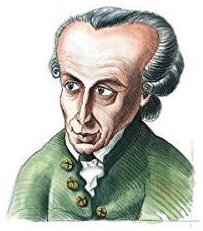
\includegraphics[width=0.4\textwidth]{images/kant/kant_a.jpg}
\end{figure}
\newpage

\tableofcontents
\newpage

\section{Teil 1}

\subsection{Das Ziel Kants}

Das Wort \emph{rein} im Titel \emph{Die Kritik der reinen Vernunft} bezieht sich auf das Freisein von Erfahrung, also der Empirie vorgreifend. Die Vernunft soll sich in diesem Werk also selbst begegnen und erkennen. Die Geistesschulen des Empirismus und des Rationalismus sind im Thema der Metaphysik, also der Erforschung der Erkenntnisse unabh"angig von aller Erfahrung, zerstritten und Kant nimmt sich in diesem Werk zum Ziel, den Streit dieser beiden Schulen auf auf gewisse Irrt"umer zur"uckzuf"uhren und wieder so vers"ohnen. Zudem soll die Wissenschaftlichkeit der Metaphysik bewiesen werden. Dies vergleicht Kant mit der kopernikanischen Revolution, welches ein Sinnbild ist das sich durch den Verlauf des Textes durchzieht.

\subsection{Das n"otige Handwerkszeug}

\begin{description}[leftmargin=!,labelwidth=\widthof{\bfseries Empirische Erkenntnis}]
  \item[Empirismus] 
  \item[Rationalismus] 
  \item[Reine Erkenntnis]
  \item[Empirische Erkenntnis]
  \item[Analytisches Urteil]
  \item[Synthetisches Urteil]
\end{description}

\newpage

\section{"Uber den Autor}
Ralf Ludwig studierte Theologie und Philosophie, promovierte über Kant, war evangelischer Pastor und unterrichtete am Gymnasium. Seit einigen Jahren lebt er als freier Schriftsteller in München.

\begin{figure}[h]
	\centering
	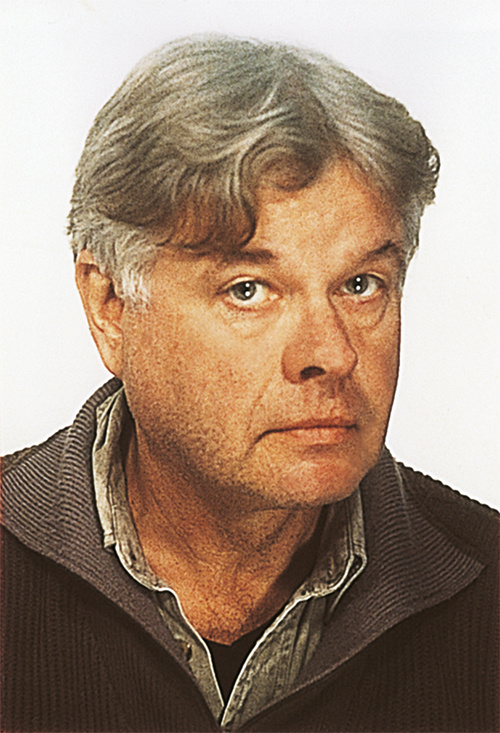
\includegraphics[width=0.3\textwidth]{images/kant/rludwig.jpg}
\end{figure}
\newpage

\end{document}
